\documentclass[12pt]{article}
\usepackage{jmlda}
% \documentclass[12pt,a4paper]{amsart}
% \usepackage[cp1251]{inputenc}
% \usepackage{graphicx}
% \usepackage{color}
% \usepackage{epstopdf} % http://tex.stackexchange.com/questions/29664/latex-error-unknown-graphics-extension-eps
% \usepackage[colorlinks,unicode,pdfpagelabels=true]{hyperref}
% \usepackage[english,russian]{babel}
% \usepackage{amssymb,enumerate}
% \usepackage{enumitem}  \setlist{nolistsep}
\usepackage{tikz}
% \usepackage{textcase} % for UTF-8 in header

%%%%%%%%%%%%%%%%%%%%%%%%%%%%%%%%%%%%%%%%%%%%%%%%%%%%%%%%%%%%
%%%%%%%%%%%%%%%%%%%% 	\input macro.tex
%%%%%%%%%%%%%%%%%%%%%%%%%%%%%%%%%%%%%%%%%%%%%%%%%%%%%%%%%%%%
	\newcommand\ol[1]{\overline{#1}}

	\def\cond{\,|\,}
	\newcommand\normal[2]{\mathcal{N}\!\cbr{#1,#2}}

	\newcommand\al[1]{\begin{align*} #1 \end{align*}}
	\newcommand\begcas[1]{\begin{cases}#1\end{cases}}

	\def\le{\leqslant}
	\def\ge{\geqslant}
	\def\Ell{\mathcal{L}}
	\def\Rn{\ensuremath{\mathbb{R}^n}}

	\newcommand\mb[1]{\ensuremath{\boldsymbol{\mathbf{#1}}}}
	% \newcommand\argmax[1]{\arg\underset{#1}\max\,} % \operatornamewithlimits
	\newcommand{\prodl}{\prod\limits}
	\newcommand{\suml}{\sum\limits}

	\newcommand\cbr[1]{\left(#1\right)} %circled brackets
	\newcommand\fbr[1]{\left\{#1\right\}} %figure brackets
	\newcommand\sbr[1]{\left[#1\right]} %square brackets
	\newcommand\modul[1]{\left|#1\right|}
	\newcommand\norm[1]{\ensuremath{\left\|{#1}\right\|}}

	% \newcommand{\T}{^{\text{\tiny\sffamily\upshape\mdseries T}}}
	\newcommand\dd[2]{\frac{\partial#1}{\partial#2}}

\begin{document}
%%%%%%%%%%%%%%%%%%%%%%%%%%%%%%%%%%%%%%%%%%%%%%%%%%%%%%%%%%%%
%%%%%%%%%%%%%%%%%%%% 			\begin{abstract}
Решается задача одноклассовой классификации электронных писем на предмет наличия в них спама. В работе вводится квазивероятностная модель для классической эмпирической постановки задачи одноклассовой классификации. Произведена модификация, позволяющая накладывать различные требования отбора признаков. Построенные методы классификации проверяются вычислительными экспериментами на модельных и реальных данных.
%Решается задача автоматического разделения текстов по тематикам. Рассмотрены два подхода к решению задачи: вероятностный латентный семантический анализ и алгоритм латентного размещения Дирихле, основанные на различных вероятностных предположениях о текстах, однако обладающие схожей вычислительной техникой. Произведено сведение алгоритмов и их модификаций к новой обобщающей вычислительной схеме и построен новый алгоритм. Проанализировано качество и скорость сходимости построенного алгоритма в зависимости от внутренних параметров и числа тем, ассоциируемых с каждым словом в тексте. Результаты подтверждены численным экспериментом на реальных текстах. 
\end{abstract}
%%%%%%%%%%%%%%%%%%%%%%%%%%%%%%%%%%%%%%%%%%%%%%%%%%%%%%%%%%%%
	\title{Вероятностная модель одноклассовой классификации}
	\author{М.\,О.\,Бурмистров, Л.\,Н.\,Сандуляну}
	\address{Московский физико-технический институт, ФУПМ, каф. <<Интеллектуальные системы>>}
	% \thanks{Научный руководитель О.\,В.\,Красоткина}
	\date{декабрь 2012\,г.}

	\begin{abstract}
	Решается задача одноклассовой классификации электронных писем на предмет наличия в них спама. 
	В работе вводится квазивероятностная модель для классической эмпирической постановки задачи одноклассовой классификации и 
	производится сведение классического подхода к новой модели.
	%Произведена модификация, позволяющая накладывать различные требования отбора признаков. 
	Построенные методы классификации проверяются вычислительными экспериментами на модельных и реальных данных.
	\end{abstract}

\maketitle
\section{Введение} 							
%%%%%%%%%%%%%%%%%%%%%%%%%%%%%%%%%%%%%%%%%%%%%%%%%%%%%%%%%%%%
%%%%%%%%%%%%%%%%%%%%		С широким развитием сети интернет и её проникновением в большую часть всех сфер жизни, у людей появилась возможность свободно обмениваться информацией и получать доступ к разнообразным ресурсом. 
Одним из наиболее распространенных способов общения людей через интернет является использование электронной почты \cite{}. 
В силу большой открытости этого канала связи с точки зрения возможности передачи любого сообщения произвольному пользователю он активно используется мошенниками, злоумышленниками и распространителями рекламных материалов. При этом создается не только повышенная нагрузка на техническую инфраструктуру, но и тратится время людей, которым приходится отделять полезную информацию, от всей остальной \cite{}. 
Поэтому задача автоматизации фильтрации электронной почты будет оставаться актуальной в течение всего времени её существования.

Задача фильтрации спама уже решалась многими методами \cite{}, однако они в большой степени являлись эвристическими и не имели под собой четкой вероятностной модели. 
Также проблемой является корректное составление обучающей выборки. 
Дело в том, что спам-письма зачастую шаблонны и имеют много общего в своей структуре, к тому же они широко доступны. 
Составить же обучающую выборку, содержащую письма, полезные для пользователей, гораздо сложнее по следующим причинам:
\begin{itemize}
	\item меньшая доступность,
	\item высокая разнородность,
	\item большое число шаблонных писем (разнообразные уведомления от сервисов).
\end{itemize}
По этим причинам предлагается использовать методы одноклассовой классификации \cite{}, чтобы отказаться от требования к обучающей выборки содержать достаточно широкой множество разнообразных представителей обоих классов.

В работе будет предложена квазивероятностная постановка задачи одноклассовой классификации. 
За счет такого подхода становятся яснее области применимости построенной модели и предъявляемые требования к данным.

Поскольку количество признаков, которые можно извлечь из текстов спам-писем, очень велико, то предлагается применить отбор признаков. 
На основе полученной вероятностной постановки задачи, строится новая вероятностная модель порождения объектов, в ходе оптимизации которой происходит требуемый отбор признаков.

Полученные методы построения одноклассовых классификаторов применяются к модельным и реальным данным.

%Современный интернет обладает широкой, распределенной и сложной архитектурой, в которой зачатую затруднительно найти новую требуемую информацию. Помочь пользователю решить задачу поиска призваны поисковые системы, которые автоматически сканируют интернет и выявляют наиболее подходящие пользователю по некоторым ключевым словам. 

%Алгоритм определения степени соответствия сайта запросу пользователя основан на множестве характеристик, а владельцы ресурсов заинтересованы, чтобы поисковые системы как можно выше оценивали их сайт. Зачастую

%Злоумышленники пытаются вывести подконтрольные им сайты в топ поисковой выдачи, искусственно изменяя характеристики сайта, видимые для поисковой машины. Такие действия ухудшают качество поиска и опасны для пользователя, поэтому необходимо либо полностью блокировать такие сайты, либо существенно опускать их в выдаче.

%Задача могла бы рассматривать как традиционная задача бинарной классификации, если бы знание поисковой машины характеристик сайта не влияло на эти характеристики. Например, если сайт признан по какой-либо причине опасным и удален из выдачи, у него резко (в разы) снижается посещаемость, при этом сайт мог исправить свою проблему, но не разбанится автоматически и посещаемость останется низкой. Одновременно с этим существуют признаки (количество переходов), которые, по-видимому, отражают степень полезность сайта, однако слабо зависят от действий поисковой системы. Задача выделения признаков, не зависящих от поисковой машины также представляет интерес в нашем исследовании.

%Идея: пусть каждый сайтовладелец в каждый момент времени $t\in T$ (см. презентацию) думает: сделать ему сайт хуже или лучше (спамерское поведение или, напротив, добропорядочное --- это и есть на самом деле класс $y\in Y$). В зависимости от этого он меняет характеристики своего сайта (тут чуть веселее, на самом деле: он одинаково меняет характеристики {\it всех} сайтов, которыми владеет, а это можно узнавать по whois-данным. {\it но я думаю, что в работе с этим заморачиваться не будем}). В таком случае наблюдаемые характеристики сайта (те, которые зависят) есть, на самом деле, функция от его наблюдаемого класса (то, что люди видят глазами). Надо додумать. Статей по теме не находил (да и не искал: придумал поздно вечером).
%%%%%%%%%%%%%%%%%%%%%%%%%%%%%%%%%%%%%%%%%%%%%%%%%%%%%%%%%%%%
	С широким развитием сети интернет и её проникновением в большую часть всех сфер жизни, у людей появилась возможность свободно обмениваться информацией и получать доступ к разнообразным ресурсом. 
	Одним из наиболее распространенных способов общения людей через интернет является использование электронной почты. 
	В силу большой открытости этого канала связи с точки зрения возможности передачи любого сообщения произвольному пользователю он активно используется мошенниками, злоумышленниками и распространителями рекламных материалов. При этом создается не только повышенная нагрузка на техническую инфраструктуру, но и тратится время людей, которым приходится отделять полезную информацию, от всей остальной. 
	Поэтому задача автоматизации фильтрации электронной почты будет оставаться актуальной в течение всего времени её существования.

	Задача фильтрации спама уже решалась многими методами \cite{Islam2007, Sun2008}, однако они в большой степени являлись эвристическими и не имели под собой четкой вероятностной модели. 
	Также проблемой является корректное составление обучающей выборки. 
	Дело в том, что спам-письма зачастую шаблонны и имеют много общего в своей структуре, к тому же они широко доступны. 
	Составить же обучающую выборку, содержащую письма, полезные для пользователей, гораздо сложнее по следующим причинам:
	\begin{itemize}
		\item меньшая доступность,
		\item высокая разнородность,
		\item большое число шаблонных писем (разнообразные уведомления от сервисов).
	\end{itemize}
	По этим причинам предлагается использовать методы одноклассовой классификации \cite{Tax2001, Khan2006}, чтобы отказаться от требования к обучающей выборки содержать достаточно широкое множество разнообразных представителей обоих классов.

	В работе предложена квазивероятностная постановка задачи одноклассовой классификации. 
	За счет такого подхода становятся яснее области применимости построенной модели и предъявляемые требования к данным.
	% Поскольку количество признаков, которые можно извлечь из текстов спам-писем, очень велико, то предлагается применить отбор признаков. 
	На основе полученной вероятностной постановки задачи, строится новая вероятностная модель порождения объектов, в ходе оптимизации которой происходит построение классификатора. %требуемый отбор признаков.

	Полученные методы построения одноклассовых классификаторов применяются к модельным и реальным данным.


\section{Байесовская постановка задачи}  	
%%%%%%%%%%%%%%%%%%%%%%%%%%%%%%%%%%%%%%%%%%%%%%%%%%%%%%%%%%%%
%%%%%%%%%%%%%%%%%%%%		Объектом исследования является множество электронных сообщений характеризуемых некоторым набором признаков.
Рассмотрим одноклассовую классификацию объектов генеральной совокупности $\Omega$.
Пусть каждый объект $\omega \in{\Omega}$  представлен точкой в линейном пространстве признаков
$\mb x(\omega)=\cbr{x^1(\omega),\ldots, x^n(\omega)} \in {\mathbb R^n}$. При этом мы изучаем лишь объекты одного класса, поэтому меткой класса объект существенно не обладает.
Тем не менее нашей задачей будет построение классификатора, который будет давать ответ $1$, если предъявленный объект лежит в множестве, и $0$ иначе.

В работе \cite{Tax2001}  предлагается строить сферический пороговый классификатор вида
$\sbr{z \le 0} $, где $z(\mb x,\mb a,R)=\norm{\mb x-\mb a}-R$ без вероятностного обоснования такого подхода. При этом в области $z(\mb x, \mb a, R) \ge 0$ значение величины $\norm{\mb x-\mb a}^2-R^2$ несёт смысл отступа $\xi$, а для объектов внутри шара отступ полагается равным 0. Для подбора значений $\mb a, R$ решается задача
\begin{equation}
	\label{min:noprob}
	F(R,\mb a, \mb \xi) = R^2 + C\sum_i\xi_i \to \min_{\mb a, R, \mb\xi},
\end{equation}
при этом здесь и далее мы полагаем, что суммирование по индексу $i$ (а в дальнейшем и $j$) означает суммирование по всем объектам обучающей выборки.

Здесь величина $C$ задает баланс между минимальным объёмом шара и наименьшим числом объектов обучающей выборки вне сферы. Пример описания объектов шаром приведен на рисунке \ref{tikz:basic}.

\addtikz{basic}{1.2}{thick,domain=-1:2}{Пример описания объектов шаром}

Будем придерживаться следующей вероятностной модели распределения объектов генеральной совокупности.
Параметрическое семейство условных плотностей распределения в признаковом пространстве имеет вид
\begin{equation}
	\label{PhiXARC}
	\varphi \cbr{ {\mb x | \mb a,R;c} } \propto
		\begcas{
			&1, 		\qquad\qquad\qquad  	\! 	z(\mb x,\mb a,R) < 0, \\
			&e^{-c \cbr{\norm{\mb x-\mb a}^2-R^2}}, 	\:	z(\mb x,\mb a,R) \ge 0.
		}
\end{equation}
Здесь величина $c$ является гиперпараметром. График данной функции плотности изображен на рисунке \ref{tikz:expon}.

\addtikz{expon}{1.2}{thick,domain=0:4}{Значение плотности распределения вдоль радиуса}

Совместную плотность распределения случайной обучающей совокупности будем понимать как плотность распределения выборки независимых реализаций
$$\Phi(\mb X|\mb a,R)=\prod_{j=1}^N \varphi(\mb x_j|\mb a,R),$$
где $\mb X=\fbr{\mb x}_{j=1}^N$.
Пусть, далее, выбрана априорная плотность совместного распределения вероятностей $\Psi(\mb a,R)$ для параметров распределения $\varphi \cbr{\mb x | \mb a,R;c}$.
Тогда апостериорная плотность распределения параметров $\mb a$ и $R$ относительно обучающей совокупности определяется формулой Байеса
\begin{equation}
	\label{Prob:aRX}
	p(\mb a,R|\mb X)
	= \frac {\Psi(\mb a,R) \Phi(\mb X|\mb a,R)}
			{\int {\Psi(\mb a',R') \Phi(\mb X|\mb a',R')d\mb a'dR'}}.
\end{equation}

Из принципа максимума плотности апостериорного распределения в пространстве параметров модели генеральной совокупности получим байесовское правило обучения
\begin{equation}
	\label{argmax:full}
	\cbr{\hat{\mb a},\hat R|\mb X} = \argmax_{\mb a,R} p(\mb a,R|\mb X)
\end{equation}

При этом решающее правило принимает вид
\begin{equation}
	\label{rule:basic}
	f(\mb x) = \sbr{\norm{\mb x - \hat{\mb a}} \le \hat R}.
\end{equation}

Поскольку знаменатель в выражении (\ref{Prob:aRX}) не зависит от целевых переменных
$$p(\mb a,R|\mb X)
	\propto \Psi(\mb a,R) \Phi(\mb X|\mb a,R)
	=  \Psi(\mb a,R) \prod_{j=1}^N \varphi(\mb x_j|\mb a,R),$$
то в задаче максимизации (\ref{argmax:full}) достаточно рассматривать только числитель
$$\cbr{\hat{\mb a},\hat R|\mb X}
	= \argmax_{\mb a,R} p(\mb a,R|\mb X)
	= \argmax_{\mb a,R} \cbr{\ln\Psi(\mb a,R) + \sum_{j=1}^N\ln\varphi(\mb x_j|\mb a,R)}. $$

Теперь покажем, что задача в такой постановке обобщает задачу (\ref{min:noprob}).
Положим, что априорное распределение параметров $\Psi(\mb a,R)$ обладает следующими свойствами:
\begin{itemize}
 	\item $\mb a$ и $R$~--- случайные независимые величины,
 	\item $\modul{R}$ --- нормально распределенная случайная величина с нулевым математическим ожиданием и дисперсией $\sigma^2$,
 	\item $\mb a$ равномерно распределено по всему пространству $\Rn$ (такое распределение будет несобственным \cite{Groot1974}).
 \end{itemize}
 Тогда совместное распределение параметров также будет несобственным
 $$\Psi(\mb a,R)\propto e^{-\frac1{2\sigma^2}R^2}.$$
 Подставим это выражение и функцию распределения из (\ref{PhiXARC})
 \begin{align}
 	\label{ProbARX_simple}
 	\ln p(\mb a,R&|\mb X)
 		=	\ln\Psi(\mb a,R) + \sum_{j=1}^N\ln\varphi(\mb x_j|\mb a,R) =\notag \\
 		&= 	-\frac{R^2}{2\sigma^2} + \sum_{i: \norm{\mb x_i - \mb a} \le R} \ln 1
 			+ \sum_{i: \norm{\mb x_i - \mb a} > R} \ln e^{-c \cbr{\norm{\mb x-\mb a}^2-R^2}}  = \notag \\
 		&= -\frac{R^2}{2\sigma^2} - \sum_{i: \norm{\mb x_i - \mb a} > R} c\cbr{\norm{\mb x_i - \mb a}^2 - R^2} = \notag \\
 		&= -\frac1{2\sigma^2}\cbr{R^2 + 2\sigma^2 c\sum_{i: \norm{\mb x_i - \mb a} > R} \cbr{\norm{\mb x_i - \mb a}^2 -R^2}} \to \max_{\mb a, R}.
 \end{align}
 Очевидно, задачи (\ref{ProbARX_simple}) и (\ref{min:noprob}) эквивалентны при $C = 2\sigma^2 c.$

%%%%%%%%%%%%%%%%%%%%%%%%%%%%%%%%%%%%%%%%%%%%%%%%%%%%%%%%%%%%
	Объектом исследования является множество электронных сообщений характеризуемых некоторым набором признаков.
	Рассмотрим одноклассовую классификацию объектов генеральной совокупности $\Omega$.
	Пусть каждый объект $\omega \in{\Omega}$  представлен точкой в линейном пространстве признаков
	$\mb x(\omega)=\cbr{x^1(\omega),\ldots, x^n(\omega)} \in {\mathbb R^n}$. При этом мы изучаем лишь объекты одного класса, поэтому меткой класса объект существенно не обладает. 
	Тем не менее нашей задачей будет построение классификатора, который будет давать ответ $1$, если предъявленный объект лежит в множестве, и $0$ иначе.

	В работе \cite{Tax2001}  предлагается строить сферический пороговый классификатор вида 
	$\sbr{z \le 0} $, где $z(\mb x,\mb a,R)=\norm{\mb x-\mb a}-R$ без вероятностного обоснования такого подхода. При этом в области $z(\mb x, \mb a, R) \ge 0$ значение величины $\norm{\mb x-\mb a}^2-R^2$ несёт смысл отступа $\xi$, а для объектов внутри шара отступ полагается равным 0. Для подбора значений $\mb a, R$ решается задача
	\begin{equation}
		\label{min:noprob}
		F(R,\mb a, \mb \xi) = R^2 + C\sum_i\xi_i \to \min_{\mb a, R, \mb\xi}.
	\end{equation}
	Здесь величина $C$ задает баланс между минимальным объёмом шара и наименьшим числом объектов обучающей выборки вне сферы. Пример описания объектов щаром приведен на рисунке \ref{eps:example}.

	%\addtikz{basic}{1.2}{thick,domain=-1:2}{Пример описания объектов шаром}
	\begin{figure} [!ht] %lrp
		\centering
		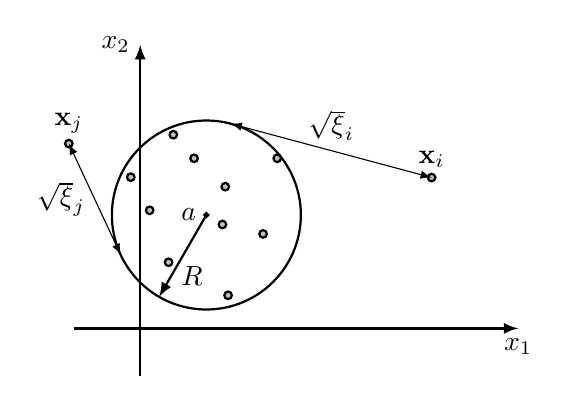
\begin{tikzpicture}[x=1.2cm,y=1.2cm,thick,domain=-1:2]
			\newcommand\cird[1]{\draw [fill = lightgray] (center) ++ (#1) circle (0.04);} %, thin]

			\node (center) at (0.7,1.2) {};
			\draw[-latex] (-0.7,0) -- (4,0) node[below] {$x_1$};
			\draw[-latex] (0,-0.5) -- (0,3) node[left] {$x_2$};
			\draw [fill = none] (center) circle (1.0);
			\draw [fill = black] (center) circle (0.02);
			\cird{0.2,0.3}
			\cird{-0.13,0.6}
			\cird{0.17,-0.1}
			\cird{0.6,-0.2}
			\cird{-0.4,-0.5}
			\cird{-0.6,0.05}
			\cird{0.23,-0.85}
			\cird{-0.35,0.85}
			\cird{-0.8,0.4}
			\cird{0.75,0.6}

			\draw[fill = lightgray] (center) ++(75:1) ++(-15:2.2)circle (0.04) node[above]{$\mb x_i$};
			\draw[latex-latex, thin] (center) ++(75:1) -- ++(-15:2.2) node[pos=0.5,above]{$\sqrt\xi_i$};

			\draw[fill = lightgray] (center) ++(205:1) ++(115:1.3)circle (0.04) node[above]{$\mb x_j$};
			\draw[latex-latex, thin] (center) ++(205:1) -- ++(115:1.3) node[pos=0.5,left]{$\sqrt\xi_j$};

			\draw[latex-] (center) ++(240:1) -- +(60:1) node[pos=0.25, right] {$R$};
			\node[left] at (center) {$a$};
		\end{tikzpicture}
		\vspace{-10pt}
		\caption{Пример описания объектов шаром}
		\label{tikz:basic}	
	\end{figure}

	Будем придерживаться вероятностной модели распределения объектов генеральной совокупности.
	Параметрическое семейство условных плотностей распределения в признаковом пространстве имеет вид 
	\begin{equation}
		\label{PhiXARC}
		\varphi \cbr{ {\mb x | \mb a,R;c} } \propto
			\begcas{
				&1, 		\qquad\qquad\qquad  	\! 	z(\mb x,\mb a,R) < 0, \\
				&e^{-c \cbr{\norm{\mb x-\mb a}^2-R^2}}, 	\:	z(\mb x,\mb a,R) \ge 0.
			} 
	\end{equation}
	Здесь величина $c$ является гиперпараметром. График данной функции плотности изображен на рисунке \ref{tikz:expon}.

	\begin{figure} [!ht] %lrp
		\centering
		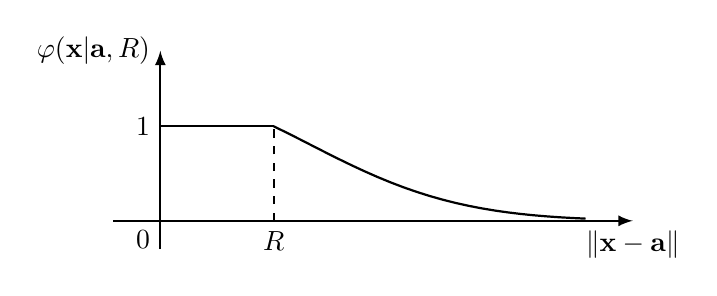
\begin{tikzpicture}[x=1.2cm,y=1.2cm,thick,domain=0:4]
			\draw[-latex] (-0.5,0) -- (5,0) node[below] {$\|\mb x-\mb a\|$};
			\draw[-latex] (0,-0.3) -- (0,1.8) node[left] {$\varphi(\mb x | \mb a, R)$};

			\draw[domain=0:1.2] plot (\x,1);
			\draw[domain=1.2:4.5] plot (\x,{exp(-0.2*(\x*\x-1.44))});
			\draw[dashed] (1.2,0) -- ++(0,1) ++(0,-1) node[below] {$R$};

			\node[left] at (0,1) {$1$};
			\node[below left] at (0,0) {$0$};
		\end{tikzpicture}
		\vspace{-10pt}
		\caption{Значение плотности распределения вдоль радиуса}
		\label{tikz:expon}	
	\end{figure}

	Совместную плотность распределения случайной обучающей совокупности будем понимать как плотность распределения выборки независимых реализаций
	$$\Phi(\mb X|\mb a,R)=\prod_{j=1}^N \varphi(\mb x_j|\mb a,R),$$ 
	где $\mb X=\fbr{\mb x}_{j=1}^N$.
	Пусть, далее, выбрана априорная плотность совместного распределения вероятностей $\Psi(\mb a,R)$ для параметров распределения $\varphi \cbr{\mb x | \mb a,R;c}$. 
	Тогда апостериорная плотность распределения параметров $\mb a$ и $R$ относительно обучающей совокупности определяется формулой Байеса
	\begin{equation}
		\label{Prob:aRX}
		p(\mb a,R|\mb X)
		= \frac {\Psi(\mb a,R) \Phi(\mb X|\mb a,R)}
				{\int {\Psi(\mb a',R') \Phi(\mb X|\mb a',R')d\mb a'dR'}}.
	\end{equation}

	Из принципа максимума плотности апостериорного распределения в пространстве параметров модели генеральной совокупности получим байесовское правило обучения
	\begin{equation}
		\label{argmax:full}
		\cbr{\hat{\mb a},\hat R|\mb X} = \argmax_{\mb a,R} p(\mb a,R|\mb X)
	\end{equation}

	Поскольку знаменатель в выражении (\ref{Prob:aRX}) не зависит от целевых переменных 
	$$p(\mb a,R|\mb X) 
		\propto \Psi(\mb a,R) \Phi(\mb X|\mb a,R) 
		=  \Psi(\mb a,R) \prod_{j=1}^N \varphi(\mb x_j|\mb a,R),$$
	то в задаче максимизации (\ref{argmax:full}) достаточно рассматривать только числитель
	$$\cbr{\hat{\mb a},\hat R|\mb X}
		= \argmax_{\mb a,R} p(\mb a,R|\mb X) 
		= \argmax_{\mb a,R} \cbr{\ln\Psi(\mb a,R) + \sum_{j=1}^N\ln\varphi(\mb x_j|\mb a,R)}. $$

	Теперь покажем, что задача в такой постановке обобщает задачу (\ref{min:noprob}). 
	Положим, что априорное распределение параметров $\Psi(\mb a,R)$ обладает следующими свойствами:
	\begin{itemize}
	 	\item $\mb a$ и $R$~--- случайные независимые величины,
	 	\item $\modul{R}$ --- нормально распределенная случайная величина с нулевым математическим ожиданием и дисперсией $\sigma^2$,
	 	\item $\mb a$ равномерно распределено по всему пространству $\Rn$ (такое распределение будет несобственным \cite{Groot1974}).
	 \end{itemize} 
	 Тогда совместное распределение параметров также будет несобственным 
	 $$\Psi(\mb a,R)\propto e^{-\frac1{2\sigma^2}R^2}.$$
	 Подставим это выражение и функцию распределения из (\ref{PhiXARC})
	 \begin{align}
	 	\label{ProbARX_simple}
	 	\ln p(\mb a,R&|\mb X) 
	 		=	\ln\Psi(\mb a,R) + \sum_{j=1}^N\ln\varphi(\mb x_j|\mb a,R) =\notag \\
	 		&= 	-\frac{R^2}{2\sigma^2} + \sum_{i: \norm{\mb x_i - \mb a} \le R} \ln 1 
	 			+ \sum_{i: \norm{\mb x_i - \mb a} > R} \ln e^{-c \cbr{\norm{\mb x-\mb a}^2-R^2}}  = \notag \\
	 		&= -\frac{R^2}{2\sigma^2} - \sum_{i: \norm{\mb x_i - \mb a} > R} c\cbr{\norm{\mb x_i - \mb a}^2 - R^2} = \notag \\
	 		&= -\frac1{2\sigma^2}\cbr{R^2 + 2\sigma^2 c\sum_{i: \norm{\mb x_i - \mb a} > R} \cbr{\norm{\mb x_i - \mb a}^2 -R^2}} \to \max_{\mb a, R}.
	 \end{align}
	 Очевидно, задачи (\ref{ProbARX_simple}) и (\ref{min:noprob}) эквивалентны при $C = 2\sigma^2 c.$


\section{Решение оптимизационной задачи} 	
%%%%%%%%%%%%%%%%%%%%%%%%%%%%%%%%%%%%%%%%%%%%%%%%%%%%%%%%%%%%
%%%%%%%%%%%%%%%%%%%%		Итак, для нахождения значений $\mb a$ и $R$ необходимо решить следующую задачу
\begin{equation}
\label{min:main}
			\begcas{
			&R^2 + C\suml_i\xi_i \to \min\limits_{\mb a, R,\mb\xi}, \\
			&\norm{\mb x_i-\mb a}^2\le R^2 + \xi_i,\quad\xi_i\ge0,\quad i = 1,\ldots,N.
			}
\end{equation}
Функция Лагранжа этой задачи имеет вид
\begin{equation*}
	\Ell(\mb a, R,\mb\xi,\mb\alpha,\mb\gamma)=
		R^2 + C\suml_i\xi_i - \suml_i\gamma_i\xi_i
		- \suml_i\alpha_i\cbr{R^2 + \xi_i - \cbr{\mb x_i\T\mb x_i - 2\mb a\T\mb x_i + \mb a\T\mb a}},
\end{equation*}
где $\alpha_i\ge 0$  и $\gamma_i\ge 0$ --- множители Лагранжа.
Необходимым условием минимума является равенство нулю частных производных функции Лагранжа по всем переменным
\begin{equation}
	\label{minLag}
	\begin{array}{ll}
		\dd \Ell R = 0: & \suml_i \alpha_i = 1 \:\cbr{\text{случай $R = 0$ рассмотрим отдельно},}\\
		\dd \Ell{\mb a} = 0: & \mb a = \cfrac{\suml_i\alpha_i\mb x_i}{\suml_i \alpha_i}= \suml_i \alpha_i\mb x_i,\\
		\dd \Ell{\xi_i} = 0: & \gamma_i = C - \alpha_i, \;\; i = 1,\ldots,N.
	\end{array}
\end{equation}

Из последнего уравнения получаем, что $\alpha_i = C - \gamma_i$.
Таким образом, мы получаем новые ограничения на $\alpha_i$
$$0\le\alpha_i\le C, \;\; i = 1,\ldots,N.$$

Если это ограничение выполнено, то мы можем вычислить $\gamma_i$ по формуле $\gamma_i = C - \alpha_i$, и при этом автоматически будет выполнено условие $\gamma_i\ge 0$.

Тогда для функции Лагранжа получим выражение
{
\newcommand\ai[0]{\alpha_i\,}
\newcommand\aj[0]{\alpha_j\,}
\newcommand\mbx[1]{\mb x_#1}
%\newcommand\cd[0]{\!\cdot\!}
\newcommand\cd[0]{\T}
\al{
\Ell(\mb a, R,&\mb\xi,\mb\alpha,\mb\gamma)
	= 	R^2 - \suml_i\ai R^2 + C\suml_i\xi_i - \suml_i\ai\xi_i  +\\
	&+ \suml_i\ai\mbx i\cd\mbx i -  2\suml_i\ai\mb a\cd\mbx i + \suml_i\ai\mb a\cd\mb a - \suml_i\gamma_i\xi_i =\\
	&= R\cd R\cd\cbr{1-\suml_i\ai} +\suml_i\xi_i\cbr{C-\ai-\gamma_i} + \\
	&+ 	\suml_i\ai\mbx i\cd\mbx i - 2 \suml_i\ai\suml_j\aj\mbx j\cd\mbx i
	+ 	\suml_{i,j}\ai\aj \mbx j\cd \mbx i = \\
	&= 	\suml_i\ai\mbx i\cd\mbx i-\suml_{i,j}\ai\aj\mbx j\cd\mbx i \to \max_{\mb\alpha}.
}
}

Полученное выражение является квадратичной формой.
Тогда его максимум находится по известным алгоритмам решения задач квадратичного программирования.
По оптимальным значениям $\mb{\alpha}$ мы сможем найти оптимальное значение центра гипершара $\mb a$ и отступов $\mb{\xi}$, используя соотношения (\ref{minLag}).

Для каждого объекта $\mb x_i$ оптимальное значение $\alpha_i$ (или же $\gamma_i = C-\alpha_i$) задает тип принадлежности объекта построенному гипершару:
\begin{itemize}
	\item $\alpha_i=0 \Rightarrow \text{объект $\mb x_i$ лежит внутри гипершара, имеет нулевой отступ};$
	\item $0<\alpha_i<C \Rightarrow \text{объект $\mb x_i$ лежит на границе гипершара, имеет нулевой отступ};$
	\item $\alpha_i=C \Rightarrow \text{объект $\mb x_i$ лежит вне гипершара, имеет ненулевой отступ}.$
\end{itemize}

%Те векторы $\mb x_i$, для которых $\alpha_i=0$ и $\gamma_i=C$, лежат внутри гиперсферы, те, для которых $0<\alpha_i<C$ и $0<\gamma_i<C$~--- на её границе, а те, для которых $\alpha_i=C$ и $\gamma_i=0$, лежат вне гиперсферы и имеют ненулевой отступ $\mb\xi$.

Радиус $R$ определяется как расстояние от центра гипершара $\mb a$ до опорных векторов, лежащих на границе гипершара.

Если же $R = 0$, то задача (\ref{min:main}) имеет вид
\begin{equation}
	\begcas{
	&C\suml_i\xi_i \to \min\limits_{\mb a, \mb\xi}, \\
	&\norm{\mb x_i-\mb a}^2\le \xi_i,\quad\xi_i\ge0,\quad i = 1,\ldots,N.
	}
\end{equation}
т.е.
\begin{equation}
			C\suml_i\norm{\mb x_i-\mb a}^2 \to \min\limits_{\mb a},
\end{equation}
а эта задача соответствует методу наименьших квадратов. Тогда $\mb a = \frac{\sum_i \mb x_i}N$.
При этом следует понимать, что значение $R=0$ обнуляет обобщающую способность нашего классификатора, поэтому следует отказываться от такого решения, если есть выбор.
Здесь же стоит отметить, что $R = 0$ обязательно, если $C < \frac1N,$ где $N$~--- число объектов в обучающей выборке, поскольку в этом случае условия на $\mb \alpha$ несовместны.

Для возможности описания данных более гибкой формой, нежели сфера, в работе \cite{Tax2001} предлагается использовать потенциальные функции \cite{Izerman1979}. Наиболее часто используемыми потенциальными функциями являются полиномиальная
$$K_p(\mb x_i, \mb x_j) = \cbr{1 + \mb x_i\T \mb x_j}^p$$
и радиальная базисная функция Гаусса (которую мы и будем в дальнейшем рассматривать)
$$K(\mb x_i, \mb x_j) = \exp\cbr{-\frac{\norm{\mb x_i - \mb x_j}^2}{2s^2}}.$$
Таким образом, чтобы получить улучшенную модель описания данных, необходимо заменить в функции Лагранжа операцию вычисления
скалярного произведения двух векторов вычислением значения потенциальной функции двух аргументов.

При таком обобщении решающее решающее правило (\ref{rule:basic}) принимает вид 
\begin{align}
	\label{rule:kernel}
	f(\mb x) 
		&= 	\sbr{\norm{\mb x-\mb a} \le R} 
		= 	\sbr{\mb x\cdot\mb x - 2\mb x\cdot\mb a + \mb a\cdot\mb a \le R^2} = \notag \\
		&= 	\sbr{\mb x\cdot\mb x - 2\mb x\cdot\cbr{\suml_{i} \alpha_i \mb x_i} + \cbr{\suml_{i} \alpha_i \mb x_i}\cdot\cbr{\suml_{i} \alpha_i \mb x_i} \le R^2} \to \notag \\
		&\to \sbr{K(\mb x,\mb x) - 2\suml_{i} \alpha_i K(\mb x, \mb x_i) + \suml_{i,j} \alpha_i\alpha_jK(\mb x_i,\mb x_j) \le R^2}.
\end{align}

Здесь оптимальное значение $R$ определяется как значение выражения $$K(\mb x,\mb x) - 2\suml_{i} \alpha_i K(\mb x, \mb x_i) + \suml_{i,j} \alpha_i\alpha_jK(\mb x_i,\mb x_j)$$ для граничных объектов ($0<\alpha_i<C$).

После такого преобразования становится неясен вероятностный смысл предложенного подхода. Для того, чтобы исправить это воспользуемся интерепретацией, изложенной в \cite{Markov}. 

Сперва сформулируем, что мы будем называть ядром. Пусть имеем некоторое пространство $\mathcal X$. Тогда для любого гильбертова пространства $\mathcal H$ и любого отображения $\phi \colon \mathcal X \to \mathcal H$ будем называть функцию $K\colon \mathcal X\times\mathcal X\to \mathrm R$ ядром, если $\foral{x,y\in \mathcal X} K(x,y) =\abr{\phi(x),\phi(y)}$. При этом пространство $\mathcal H$ называют спрямляющим для ядра $K$.

В \cite{Steinwart} приводится доказательство того, что радиальная базисная функция Гаусса действительно является ядром, а также явно приводится вид спрямляющего пространства.

Таким образом, вероятностная интерпретация следующая. Существует некоторая генереальная совокупность объектов $\Omega$, их признаковое описание в пространстве $\mathcal X$ и отображение $\phi$ из $\mathcal X$ в гильбертово пространство $\mathcal H$. В пространстве $\mathcal H$ над $\phi(\mathcal X)$ случайно порождается распределение согласно \label{PhiXARC}:
\begin{equation}
	\label{PhiHARC}
	\varphi \cbr{ {\mb h | \mb a,R;c} } \propto
		\begcas{
			&1, 		\qquad\qquad\qquad  	\! 	z(\mb h,\mb a,R) < 0, \\
			&e^{-c \cbr{\norm{\mb h-\mb a}^2-R^2}}, 	\:	z(\mb h,\mb a,R) \ge 0.
		}
\end{equation}
где величины $\mb a$ и $R$ случайно выбираются из априорного распределения параметров $\Psi(\mb a,R)$ полностью аналогично случаю без использования ядер \ref{PsiAR}.

%%%%%%%%%%%%%%%%%%%%%%%%%%%%%%%%%%%%%%%%%%%%%%%%%%%%%%%%%%%%
	Итак для нахождения значений $\mb a$ и $R$ необходимо решить следующую задачу
	\begin{equation}
	\label{min:main}
				\begcas{
				&R^2 + C\suml_i\xi_i \to \min\limits_{\mb a, R,\mb\xi}, \\
				&\norm{\mb x_i-\mb a}^2\le R^2 + \xi_i,\quad\xi_i\ge0,\quad i = 1,\ldots,N.
				} 
	\end{equation}
	Функция Лагранжа этой задачи имеет вид
	\begin{multline*}
		\Ell(\mb a, R,\mb\xi,\mb\alpha,\mb\gamma)=
			R^2 + C\suml_i\xi_i - \suml_i\gamma_i\xi_i  -\\
		-\suml_i\alpha_i\cbr{R^2 + \xi_i - \cbr{\mb x_i\cdot\mb x_i - 2\mb a\cdot\mb x_i + \mb a\cdot\mb a}},
	\end{multline*}
	где $\alpha_i\ge 0$  и $\gamma_i\ge 0$ --- множители Лагранжа.
	Необходимым условием минимума является равенство нулю частных производных функции Лагранжа по всем переменным
	\begin{equation}
		\label{minLag}
		\begin{array}{ll}
			\dd \Ell R = 0: & \suml_i \alpha_i = 1 \:\cbr{\text{случай $R = 0$ рассмотрим отдельно,}}\\
			\dd \Ell{\mb a} = 0: & \mb a = \cfrac{\suml_i\alpha_i\mb x_i}{\suml_i \alpha_i}= \suml_i \alpha_i\mb x_i,\\
			\dd \Ell{\xi_i} = 0: & \gamma_i = C - \alpha_i, \;\; i = 1,\ldots,N.
		\end{array}
	\end{equation}

	Из последнего уравнения получаем, что $\alpha_i = C - \gamma_i$. 
	Таким образом, мы получаем новые ограничения на $\alpha_i$ 
	$$0\le\alpha_i\le C, \;\; i = 1,\ldots,N.$$

	Если это ограничение выполнено, то мы можем вычислить $\gamma_i$ по формуле $\gamma_i = C - \alpha_i$, и при этом автоматически будет выполнено условие $\gamma_i\ge 0$.

	Тогда для функции Лагранжа получим выражение
	{
	\newcommand\ai[0]{\alpha_i\,}
	\newcommand\aj[0]{\alpha_j\,}
	\newcommand\mbx[1]{\mb x_#1}
	\newcommand\cd[0]{\!\cdot\!}
	\al{
	\Ell(\mb a, R,&\mb\xi,\mb\alpha,\mb\gamma)
		= 	R^2 - \suml_i\ai R^2 + C\suml_i\xi_i - \suml_i\ai\xi_i  +\\
		&+ \suml_i\ai\mbx i\cd\mbx i -  2\suml_i\ai\mb a\cd\mbx i + \suml_i\ai\mb a\cd\mb a - \suml_i\gamma_i\xi_i =\\
		&= R\cd R\cd\cbr{1-\suml_i\ai} +\suml_i\xi_i\cbr{C-\ai-\gamma_i} + \\
		&+ 	\suml_i\ai\mbx i\cd\mbx i - 2 \suml_i\ai\suml_j\aj\mbx j\cd\mbx i
		+ 	\suml_{i,j}\ai\aj \mbx j\cd \mbx i = \\
		&= 	\suml_i\ai\mbx i\cd\mbx i-\suml_{i,j}\ai\aj\mbx j\cd\mbx i \to \max_{\mb\alpha}.
	}
	}

	Полученное выражение является квадратичной формой. 
	Тогда его максимум находится по известным алгоритмам решения задач квадратичного программирования. 
	По оптимальным значениям $\mb{\alpha}$ мы сможем найти оптимальное значение центра гиперсферы $\mb a$ и отступов $\mb{\xi}$ используя соотношения (\ref{minLag}). 
	Те векторы $\mb x_i$, для которых $\alpha_i=0$ и $\gamma_i=C$, лежат внутри гиперсферы, те , для которых $0<\alpha_i<C$ и $0<\gamma_i<C$~--- на её границе, а те, для которых $\alpha_i=C$ и $\gamma_i=0$, лежат вне гиперсферы и имеют ненулевой отступ $\mb\xi$. 
	Радиус $R$ определяется как расстояние от центра гиперсферы $\mb a$ до опорных векторов лежащих на границе гиперсферы.

	Если же $R = 0$, то задача (\ref{min:main}) имеет вид 
	\begin{equation}
				\begcas{
				&C\suml_i\xi_i \to \min\limits_{\mb a, \mb\xi}, \\
				&\norm{\mb x_i-\mb a}^2\le \xi_i,\quad\xi_i\ge0,\quad i = 1,\ldots,N.
				} 
	\end{equation}
	т.е.
	\begin{equation}
				C\suml_i\norm{\mb x_i-\mb a}^2 \to \min\limits_{\mb a},
	\end{equation} 
	а эта задача соответствует методу наименьших квадратов. Тогда $\mb a = \frac{\sum_i \mb x_i}N$. 
	При этом следует понимать, что значение $R=0$ обнуляет обобщающую способность нашего классификатора, поэтому следует отказываться от такого решения, если есть выбор. 
	Здесь же стоит отметить, что $R = 0$ обязательно, если $C < \frac1N,$ где $N$~--- число объектов в обучающей выборке, поскольку в этом случае условия на $\mb \alpha$ несовместны.

	Для возможности описания данных более гибкой формой, нежели сфера, в работе \cite{Tax2001} предлагается использовать потенциальные функции \cite{Izerman1979}. Наиболее часто используемыми потенциальными функциями являются полиномиальная
	$$K_p(\mb x_i, \mb x_j) = \cbr{1 + \mb x_i \cdot \mb x_j}^p$$
	и радиальная базисная функция Гаусса
	$$K(\mb x_i, \mb x_j) = \exp\cbr{-\frac{\norm{\mb x_i - \mb x_j}^2}{2s^2}}.$$
	Таким образом, чтобы получить улучшенную модель описания данных, необходимо заменить в функции Лагранжа операцию вычисления
	скалярного произведения двух векторов вычислением значения потенциальной функции двух аргументов.


\section{Численный эксперимент} 		 	
%%%%%%%%%%%%%%%%%%%%%%%%%%%%%%%%%%%%%%%%%%%%%%%%%%%%%%%%%%%%
%%%%%%%%%%%%%%%%%%%%		Для оценки качества работы алгоритма, следуя работе \cite{Romanenko2012}, будем измерять качество одноклассовой класификации в терминах точности и полноты.
В нашем случае точность (precision, $P$)~--- доля верно классифицированных объектов тестовой выборки среди всех объектов, отнесенных алгоритмом к единственному классу.
Полнота (recall, $R$)~--- доля верно классифицированных объектов тестовой выборки среди всех объектов, принадлежащих к единственному классу.
Более высокие значения точности и полноты соответствуют лучшему качеству классификации.
В качестве агрегированного показателя, объединяющего точность $P$ и полноту $R$ используем $F_1$-меру \cite{Rijsbergen1979}:
$$F_1 = \frac{2PR}{P+R}.$$
%Большим значениям $P$ и $R$ соотвтествую

Для проведения вычислительного эксперимента\footnote{Код доступен по адресу \textsf{https://github.com/burmisha/daml/tree/master/9\_term/aspam}} на модельных данных
сгенерируем $N=400$ случайных точек $\fbr{\mb x_i}_{i=1}^N$ из распределения (\ref{PhiXARC}) 
при размерности пространства $n=2$ (для наглядности), положив направления смещений случайными и придав параметрам значения $\mb a = \cbr{1,2}\T, R = 3, c = 0{,}2.$
После этого проведем $t{\times}q$-fold кросс-валидацию с $t = 10, q = 3$, скользящим контролем подбирая параметр $C$ по значению $F_1$-метрики.
При этом все объекты, лежащие вне сферы с центром $\hat{\mb a}$ и радиуса $\hat R$, мы считаем не принадлежащим классу, 
а все объекты внутри неё~--- считаем, поскольку нашей задачей является именно поиск этой гиперсферы.

На рисунке \ref{tikz:CV} изображена полученная зависимость значения $F_1$-метрики от параметра $C$.
Из графика видно, что при $C\to 0$ обобщающая способность стремится к нулю, поскольку практически отсутствует штраф за непопадание в класс при обучении.
При этом большие штрафы заставляют необоснованно увеличивать сферу, снижая точность.

Пример работы алгоритма приведен на рисунке \ref{tikz:workexample} при параметрах $n=2, N=400, R=3, \mb a = \cbr{1,2}\T, C = 0{,}007.$ Здесь 2-мерная сфера строилась по всем объектам.
Зеленым изображена граница истинного распределения, красным~--- построенного.
Видно, что здесь $C$ оказалось слишком мало и сфера получилось описывает лишь небольшую часть объектов.

\begin{figure}[h]
	\centering
	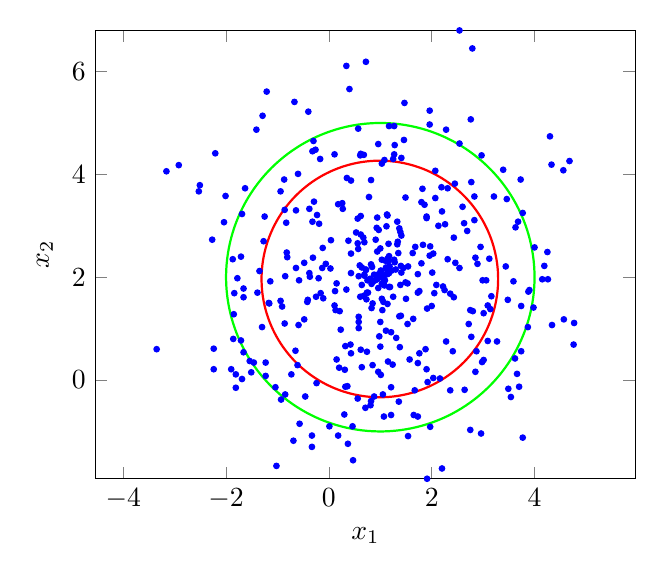
\begin{tikzpicture}
		\begin{axis}[xlabel=$x_1$, ylabel=$x_2$, enlargelimits=false, scaled ticks=false,axis equal=true]
			\addplot +[green, mark=none, domain=0:360,samples=180, thick]({1 + 3*cos(x)},{2+3*sin(x)});
			\addplot [blue, only marks, mark size=1pt]  coordinates {
			 (3.62,0.42)(-1.30,1.03)(0.12,1.73)(2.20,3.28)(-0.41,1.56)(0.36,-0.12)(-1.04,-0.14)(0.64,1.85)(-1.66,0.54)(-1.51,0.15)(-0.25,1.62)(0.43,0.52)(-0.83,3.06)(2.36,-0.20)(-1.71,2.40)(3.63,2.97)(0.42,0.69)(-0.58,1.94)(-2.53,3.67)(2.77,0.84)(4.15,1.96)(1.37,2.95)(1.67,-0.20)(2.31,3.73)(-2.21,4.41)(0.72,2.15)(-0.85,2.02)(0.31,0.20)(1.30,2.15)(2.75,-0.97)(3.73,3.90)(1.49,3.55)(-1.87,2.35)(1.53,1.88)(2.16,0.03)(0.58,1.13)(1.86,3.41)(1.96,4.97)(1.33,2.64)(2.03,2.46)(0.64,0.25)(0.62,3.19)(1.27,4.94)(-3.35,0.60)(1.35,2.47)(1.00,1.13)(3.27,0.75)(-0.38,2.08)(-1.02,-1.67)(0.34,6.11)(-1.27,2.70)(4.19,2.22)(1.90,3.18)(2.07,4.07)(-2.92,4.18)(-0.86,1.10)(4.57,1.18)(-0.87,3.90)(2.28,0.75)(2.87,0.56)(-1.69,0.02)(1.73,2.06)(1.90,3.15)(2.79,6.45)(2.43,1.61)(3.09,0.76)(1.47,5.39)(2.54,6.80)(2.83,3.57)(0.74,1.70)(1.03,1.87)(1.08,4.28)(-0.64,3.30)(4.33,4.19)(1.65,-0.68)(3.44,2.21)(0.20,0.24)(1.39,2.88)(4.76,0.69)(2.99,1.94)(1.07,1.92)(-0.60,4.01)(2.69,2.90)(0.83,1.87)(-0.33,-1.08)(1.31,0.82)(1.80,2.27)(1.41,2.09)(0.98,0.85)(1.37,1.24)(-1.39,1.70)(1.17,2.18)(2.01,2.09)(1.11,0.96)(0.37,-1.24)(0.18,3.42)(3.74,1.44)(3.14,1.38)(3.46,3.52)(1.03,1.58)(4.30,4.74)(-1.63,3.73)(1.17,2.08)(0.85,0.29)(0.04,2.72)(2.45,3.82)(1.40,1.25)(2.83,3.11)(-1.17,1.50)(2.03,0.04)(1.88,0.60)(0.88,2.05)(0.82,3.89)(0.32,0.66)(1.28,2.29)(-0.48,1.18)(1.80,3.46)(2.95,2.59)(-1.71,0.77)(0.96,4.59)(4.26,1.96)(1.14,2.13)(1.76,1.73)(1.57,0.40)(-2.51,3.79)(0.57,4.89)(1.76,0.52)(2.22,1.82)(1.11,2.19)(-0.46,-0.32)(2.07,3.54)(0.91,2.73)(-0.19,3.04)(0.83,1.40)(-1.78,1.98)(-0.31,2.38)(-1.41,4.87)(0.97,2.06)(1.97,-0.91)(1.25,4.30)(-0.94,1.54)(0.56,-0.36)(1.21,-0.68)(1.16,2.31)(4.25,2.49)(1.03,2.04)(-0.06,2.26)(1.16,2.65)(0.47,-1.56)(0.75,1.94)(-1.14,1.92)(-1.35,2.12)(0.61,4.37)(-2.04,3.07)(0.80,1.97)(2.54,4.60)(-0.29,3.47)(-0.73,0.11)(1.63,2.47)(1.90,0.21)(3.59,1.92)(2.20,-1.72)(1.15,0.36)(0.72,2.14)(0.96,1.79)(0.88,-0.32)(-1.23,0.08)(0.71,-0.54)(2.25,1.75)(-0.67,5.41)(2.80,1.34)(4.77,1.11)(1.19,1.81)(1.34,2.69)(-1.84,1.69)(-0.40,5.22)(3.68,3.08)(1.91,1.39)(1.00,2.56)(2.28,4.87)(3.88,1.72)(1.12,2.99)(0.67,2.77)(-0.11,1.59)(-0.93,-0.38)(3.77,3.25)(2.60,3.37)(2.19,3.75)(1.53,1.09)(-0.17,4.30)(1.17,4.94)(2.26,3.03)(-0.64,2.18)(1.24,0.30)(1.64,1.19)(0.81,-0.49)(3.70,-0.13)(4.34,1.07)(0.30,-0.67)(0.93,2.96)(0.11,4.39)(1.06,1.52)(1.25,1.62)(0.34,1.76)(1.14,1.48)(3.09,1.45)(1.18,2.21)(3.98,1.41)(-1.66,1.78)(-0.69,-1.18)(1.73,0.33)(0.82,-0.41)(-2.27,2.73)(-0.91,1.43)(1.83,2.63)(-1.21,5.61)(1.12,2.06)(-0.20,1.98)(3.77,-1.12)(1.00,0.65)(-0.13,2.18)(1.17,2.41)(-2.24,0.61)(1.49,1.90)(1.13,3.22)(-2.01,3.58)(-0.59,1.07)(-0.86,3.31)(3.12,2.36)(2.98,0.35)(1.01,2.11)(2.72,1.09)(0.90,1.94)(4.00,2.58)(-0.12,2.57)(1.54,-1.09)(0.62,2.83)(1.21,-0.14)(-2.24,0.21)(1.08,1.84)(1.14,2.14)(1.07,1.97)(3.48,1.56)(1.03,4.21)(0.58,2.02)(-1.85,1.28)(1.05,-0.28)(1.17,1.81)(1.22,2.13)(0.73,1.57)(3.90,1.75)(1.03,2.34)(0.58,1.23)(1.68,2.59)(1.14,2.36)(0.18,-1.08)(3.01,0.39)(3.21,3.57)(0.68,4.38)(1.82,3.72)(1.14,3.20)(1.36,-0.42)(1.27,2.34)(0.61,1.62)(0.94,1.96)(1.91,-1.92)(4.56,4.08)(0.60,2.23)(-0.23,3.21)(0.62,4.40)(0.58,1.01)(-0.26,4.48)(3.06,1.94)(0.78,3.56)(0.53,2.87)(-0.32,4.45)(-1.90,0.21)(-1.66,1.61)(-0.48,2.28)(0.40,5.66)(0.38,2.71)(0.43,3.88)(-1.29,5.14)(0.03,2.17)(0.97,2.92)(2.96,-1.04)(0.84,2.20)(2.09,1.85)(-0.65,0.57)(0.69,2.68)(-0.61,0.29)(0.46,-0.90)(-0.81,2.39)(-0.24,-0.06)(-0.85,-0.28)(0.15,1.88)(-1.16,1.49)(1.39,1.85)(2.89,2.26)(3.74,0.56)(-0.33,-1.30)(0.96,0.16)(0.21,1.34)(1.27,4.39)(-1.81,-0.15)(-0.82,2.48)(0.72,6.19)(0.43,2.46)(0.64,2.19)(2.05,1.69)(0.62,0.59)(2.54,2.18)(2.00,1.44)(-0.94,3.67)(1.10,2.32)(2.46,2.28)(1.21,0.93)(1.33,3.08)(0.76,1.70)(3.16,1.63)(0.11,1.45)(0.43,2.08)(1.00,2.00)(1.96,2.42)(0.35,3.93)(-0.57,-0.85)(1.14,2.06)(3.54,-0.33)(1.45,2.18)(2.97,4.37)(-0.30,4.65)(2.76,5.07)(0.94,2.50)(2.75,1.36)(-0.42,1.52)(1.04,1.36)(3.01,1.30)(0.32,-0.13)(0.56,2.66)(-0.38,3.33)(-3.16,4.06)(0.15,0.40)(2.77,3.85)(0.27,3.33)(1.01,2.13)(0.13,1.36)(-1.69,3.23)(0.23,0.98)(0.82,2.25)(2.85,2.38)(2.31,2.35)(2.64,-0.19)(2.63,3.05)(-1.46,0.34)(-1.54,0.37)(0.57,2.55)(1.40,2.22)(3.87,1.03)(1.41,4.32)(0.99,2.06)(-1.81,0.11)(1.01,0.10)(2.41,0.56)(1.92,-0.04)(1.73,-0.71)(3.39,4.09)(1.38,0.64)(0.69,2.05)(1.07,-0.71)(0.56,3.14)(-1.86,0.80)(-0.37,2.01)(0.01,-0.90)(1.50,1.58)(0.68,1.64)(3.49,-0.17)(0.86,1.92)(-1.25,3.18)(1.46,4.67)(0.26,3.44)(2.36,1.68)(4.68,4.26)(0.74,0.55)(2.43,2.77)(1.54,2.21)(-0.16,1.69)(0.94,3.16)(1.96,5.24)(1.41,2.81)(1.97,2.60)(2.13,3.00)(2.85,0.16)(0.85,1.49)(3.66,0.12)(0.69,2.03)(-0.32,3.08)(1.09,1.94)(-1.23,0.34)(1.28,4.57)(1.73,1.70)
		};
		\addplot+[red,  mark=none, domain=0:360,samples=180, thick]({0.9909 + 2.3010*cos(x)},{1.9660+2.3010*sin(x)});
		\end{axis}
	\end{tikzpicture}
	\caption{Пример результата работы алгоритма при $C = 0{,}007.$}
	\label{tikz:workexample}
\end{figure}

Примеры работы алгоритма при использовании ядер приведены на рисунках \ref{eps:example_rbf_1}, \ref{eps:example_rbf_10}.
\addeps{example_rbf_1}{РБФ Гаусса: $C = 0{,}015, s=1.$}
\addeps{example_rbf_10}{РБФ Гаусса: $C = 0{,}015, s=10.$}

Эксперимент на реальных данных был проведен с использованием данных, находящихся в открытом доступе\footnote{UCI Machine Learning Repository \textsf{http://archive.ics.uci.edu/ml/datasets/Spambase}}. 
Эти данные содержат уже вычисленные признаки сообщений.
Использованная база в себе как объекты, относящиеся к спаму, так и не относящиеся.
Каждый из $n = 57$ признаков документов линейно отображался в отрезок $[0, 1]$, чтобы учесть различие в их масштабах. 
Для обучения бралась небольшая часть спам-документов (200 из ~1800).
Затем по новым точкам ним строилась сфера (в 57-мерном пространстве).
В эксперименте контрольная выборка содержала все доступные объекты (в том числе объекты из обучения). 
Для каждого из объектов контрольной выборки проверялось попадание в построенную сферу и далее вычислялась $F_1$-метрика.
Отдельно стоит отметить, что в контроле участвуют как объекты из исследуемого класса (спам-сообщений), так и не из него, хотя обучение происходило только на объектах целевого класса.
Результаты подбора параметра $C$ изображены на рисунке (\ref{tikz:CV}). Данные усреднены по 20 случайным выборкам без повторений по 200 объектов из 1800.

\begin{figure}[h]
	\begin{minipage}[h]{0.5\linewidth}
		\centering % Model_N400_0.0150-0.0005-0.0450_T20_Q3
		\begin{tikzpicture}%[x=3cm,y=3cm]
			\begin{axis}[xlabel=$C$, ylabel=$F_1$, enlargelimits=false,title={Модельные данные},
			scaled x ticks=false,xticklabel style={/pgf/number format/fixed, /pgf/number format/precision=3}]
			%_CV_Model_N400_0.0150-0.0005-0.0450_T20_Q3
			\addplot[red, mark=none, thick] coordinates {
				(0.0150, 0.9302)(0.0155, 0.9363)(0.0160, 0.9388)(0.0165, 0.9435)(0.0170, 0.9447)(0.0175, 0.9451)(0.0180, 0.9474)(0.0185, 0.9506)(0.0190, 0.9513)(0.0195, 0.9567)(0.0200, 0.9590)(0.0205, 0.9617)(0.0210, 0.9653)(0.0215, 0.9673)(0.0220, 0.9710)(0.0225, 0.9734)(0.0230, 0.9767)(0.0235, 0.9775)(0.0240, 0.9780)(0.0245, 0.9785)(0.0250, 0.9819)(0.0255, 0.9833)(0.0260, 0.9816)(0.0265, 0.9823)(0.0270, 0.9841)(0.0275, 0.9837)(0.0280, 0.9852)(0.0285, 0.9836)(0.0290, 0.9842)(0.0295, 0.9841)(0.0300, 0.9836)(0.0305, 0.9827)(0.0310, 0.9823)(0.0315, 0.9826)(0.0320, 0.9831)(0.0325, 0.9818)(0.0330, 0.9813)(0.0335, 0.9812)(0.0340, 0.9831)(0.0345, 0.9830)(0.0350, 0.9819)(0.0355, 0.9825)(0.0360, 0.9825)(0.0365, 0.9809)(0.0370, 0.9810)(0.0375, 0.9785)(0.0380, 0.9806)(0.0385, 0.9805)(0.0390, 0.9805)(0.0395, 0.9806)(0.0400, 0.9806)(0.0405, 0.9802)(0.0410, 0.9805)(0.0415, 0.9797)(0.0420, 0.9789)(0.0425, 0.9782)(0.0430, 0.9795)(0.0435, 0.9779)(0.0440, 0.9781)(0.0445, 0.9783)(0.0450, 0.9782)
			};
			%\legend{$\ln Iter$, $\ln n!$}
			\end{axis}
		\end{tikzpicture}
  	\end{minipage}
	\hfill
  	\begin{minipage}[h]{0.5\linewidth}
		\centering
		\begin{tikzpicture}%[x=3cm,y=3cm]
			\begin{axis}[xlabel=$C$, ylabel=$F_1$, title={Реальные данные},
						 scaled ticks=false, enlargelimits=false,
						 xticklabel style={/pgf/number format/fixed, /pgf/number format/precision=3},
						 yticklabel style={/pgf/number format/fixed, /pgf/number format/precision=3}
						]
			%_CV_Real_N200_0.0300-0.0050-0.1500_T20
			\addplot[red, mark=none, thick] coordinates {
				(0.0300, 0.7311)(0.0350, 0.7365)(0.0400, 0.7388)(0.0450, 0.7409)(0.0500, 0.7415)(0.0550, 0.7426)(0.0600, 0.7418)(0.0650, 0.7415)(0.0700, 0.7404)(0.0750, 0.7394)(0.0800, 0.7376)(0.0850, 0.7370)(0.0900, 0.7368)(0.0950, 0.7363)(0.1000, 0.7357)(0.1050, 0.7349)(0.1100, 0.7344)(0.1150, 0.7338)(0.1200, 0.7337)(0.1250, 0.7335)(0.1300, 0.7338)(0.1350, 0.7335)(0.1400, 0.7333)(0.1450, 0.7330)(0.1500, 0.7330)
			};
			\end{axis}
		\end{tikzpicture}
	\end{minipage}
	\caption{Зависимость $F_1$-метрики от параметра регуляризации $C$}
	\label{tikz:CV}
\end{figure}

% \addeps{CrValLong}{Модельные данные. Зависимость $F_1$-метрики от параметра регуляризации $C$.}  % CV_0.000-0.010-0.200_T10_Q3.eps
% \addeps{example}{Пример результата работы алгоритма при $C = 0{,}007.$}

В обоих экспериментах отчетливо прослеживаются максимумы метрики, что свидетельствует о наличии в обеих задачах оптимального значения параметра $C.$

Результат при использовании ядра Гаусса получаем изображен на рисунке \ref{tikz:CV_rbf}.

\begin{figure}[h]
	\centering 
	\begin{tikzpicture}%[x=3cm,y=3cm]
		\begin{axis}[xlabel=$C$, ylabel=$F_1$, title={Реальные данные},
					 scaled ticks=false, enlargelimits=false,
					 xticklabel style={/pgf/number format/fixed, /pgf/number format/precision=3},
					 yticklabel style={/pgf/number format/fixed, /pgf/number format/precision=3}
					]
			%_CV_Real_N300_0.0400-0.0040-0.1200_T20_rbf0.700
			\addplot[red, mark=none, thick] coordinates {
				(0.040,0.7450)(0.044,0.7443)(0.048,0.7475)(0.052,0.7465)(0.056,0.7468)(0.060,0.7469)(0.064,0.7463)(0.068,0.7482)(0.072,0.7480)(0.076,0.7489)(0.080,0.7439)(0.084,0.7487)(0.088,0.7462)(0.092,0.7439)(0.096,0.7485)(0.100,0.7480)(0.104,0.7481)(0.108,0.7469)(0.112,0.7486)(0.116,0.7464)(0.120,0.7469)
			};
		\end{axis}
	\end{tikzpicture}
	\caption{Зависимость $F_1$-метрики от $C$ при РБФ Гаусса с $s = 0.7$}
	\label{tikz:CV_rbf}
\end{figure}

Видно, что результаты не столь устойчивы, однако они стабильно выше разультатов обычного алгоритма в достаточно широком диапозоне параметра регуляризации. Этот факт позволяет судить об эффективности предложенного подхода.

%%%%%%%%%%%%%%%%%%%%%%%%%%%%%%%%%%%%%%%%%%%%%%%%%%%%%%%%%%%%
	Для оценки качества работы алгоритма предлагается ввести метрику. 
	Следуя работе  \cite{Romanenko2012}, будем измерять качество одноклассовой класификации в терминах точности и полноты. 
	В нашем случае точность (precision)~--- доля верно классифицированных объектов тестовой выборки среди всех объектов, отнесенных алгоритмом к единственному классу. 
	Полнота (recall)~--- доля верно классифицированных объектов тестовой выборки среди всех объектов, принадлежащих к единственному классу. 
	Более высокие значения точности и полноты соответствуют лучшему качеству классификации. 
	В качестве агрегированного показателя, объединяющего точность $P$ и полноту $R$ используем $F_1$-меру \cite{Rijsbergen1979}:
	$$F_1 = \frac{2PR}{P+R}.$$

	Для проведения вычислительного эксперимента сгенерируем $N=400$ случайных точек $\fbr{\mb x_i}_{i=1}^N$ из распределения (\ref{PhiXARC}) при размерности пространства $2$ (для наглядности), положив направления смещений случайными и придав параметрам значения $a = \cbr{1,2}\T, R = 3, c = 0{,}2.$
	После этого проведем $t{\times}q$-fold кросс-валидацию с $t = 10, q = 3$, скользящим контролем подбирая параметр $C$ и вычисляя $F_1$-метрику при каждом его значении. При этом всё, что лежит вне сферы мы считаем не принадлежащим классу, а всё, что внутри,~--- считаем.
	В результате получим следующую зависимость значения метрики от $C$ (см. рисунок \ref{eps:CrValLong}).
	Из графика видно, что при $C\to 0$ обобщающая способность также стремится к нулю, поскольку практически отсутствует штраф за непопадание в класс при обучении. 
	При этом большие штрафы заставляют необоснованно увеличивать сферу, снижая точность.

	Пример работы алгоритма приведен на рисунке \ref{eps:example} при параметре $C = 0{,}007.$ 
	Зеленым изображена граница истинного распределения, красным~--- построенного.
	Видно, что здесь $C$ слишком мало и сфера получилось слишком маленькой, поскольку штраф за .
	
	\begin{figure}[!ht] %lrp
		\centering
		\includegraphics[height=240px]{CrValLong.eps} % CV_0.000-0.010-0.200_T10_Q3.eps
		\vspace{-5pt}
		\caption{Модельные данные. Зависимость $F_1$-метрики от параметра регуляризации $C$.}
		\label{eps:CrValLong}
	\end{figure}

	\begin{figure}[!ht] %lrp
		\centering
		\includegraphics[height=240px]{example.eps} 
		\vspace{-5pt}
		\caption{Пример результата работы алгоритма при $C = 0{,}007.$}
		\label{eps:example}
	\end{figure}

	Для проведения эксперимента на реальных данных были выбраны доступные в открытом доступе уже вычисленные признаки сообщений \footnote{UCI Machine Learning Repository \href{http://archive.ics.uci.edu/ml/datasets/Spambase}{http://archive.ics.uci.edu/ml/datasets/Spambase}}. 
	Здесь для обучения бралась небольшая часть спам-документов (200 из ~1800). 
	Сперва они линейно отображались в куб $[0, 1]^k$ ($k = 57$~--- размерность пространства), а затем по ним строилась сфера в этом 57-мерном пространстве. 
	Для контроля все остальные данные преобразовывались по тому же правилу (что не гарантирует их попадание в этот же куб), после чего проверялось попадание в построенную сферу и вычислялась $F_1$-метрика. 
	Здесь в контроле уже участвуют объекты как объекты из исследуемого класса (спам-сообщений), так и не из него, хотя обучение происходило только на объектах целевого класса. 
	Результаты подбора параметра $C$ изображены на рисунке (\ref{eps:CVReal}). Данные усреднены по 20 случайным выборкам по 200 объектов из 1800.

	\begin{figure}[!ht] %lrp
		\centering
		\includegraphics[height=240px]{CVReal.eps} % Real_N200_0.0300-0.0050-0.1500_T20.eps
		\vspace{-5pt}
		\caption{Реальные данные. Зависимость $F_1$-метрики от параметра регуляризации $C.$}
		\label{eps:CVReal}
	\end{figure}

	В обоих экспериментах отчетливо прослеживаются максимумы метрики, что свидетельствует о наличии в обеих задачах оптимального значения параметра $C.$


\section{Заключение}						
%%%%%%%%%%%%%%%%%%%%%%%%%%%%%%%%%%%%%%%%%%%%%%%%%%%%%%%%%%%%
%%%%%%%%%%%%%%%%%%%%		В работе был предложен вероятностный подход к задаче одноклассовой классификации. Такой подход более удобен, чем классический подход, основанный на эвристических соображениях, и с теоретической, и с практической точек зрения, поскольку несет в себе ясную возможность модификаций. При этом классический подход является частным случаем предложенного алгоритма.

В работе построен алгоритм описания классов шарами, проведено его обобщения на случай ядерных функций. Проведены вычислительные эксперименты на модельных и реальных данных.
%%%%%%%%%%%%%%%%%%%%%%%%%%%%%%%%%%%%%%%%%%%%%%%%%%%%%%%%%%%%
	В работе был предложен вероятностный подход к задаче одноклассовой классификации. Такой подход более удобен, чем классический подход, основанный на эвристических соображениях, и с теоретической, и с практической точек зрения, поскольку несет в себе ясную возможность модификаций. При этом классический подход является частным случаем предложенного алгоритма.

	В работе построен алгоритм описания классов шарами, проведено его обобщения на случай ядерных функций. Проведены вычислительные эксперименты на модельных и реальных данных.


%%%%%%%%%%%%%%%%%%%%%%%%%%%%%%%%%%%%%%%%%%%%%%%%%%%%%%%%%%%%
%%%%%%%%%%%%%%%%%%%%		\begin{thebibliography}{99}

\bibitem{Tax2001} D.\,Tax  \textit{One-class classification; Concept-learning in the absence of
counterexamples}, Ph.D thesis, 2001.
\bibitem{Khan2006} S.\,Khan, G.\,Madden\textit{A Survey of Recent Trends in One Class
Classiffcation}, College of Engineering and Informatics, National University of Ireland Galway,
Ireland, 2006.
\bibitem{Islam2007} R.\,Islam, U.\,Chowdhury \textit{Spam filtering using ML algorithms}, Universitetets Okonomiske Institute, IADIS International Conference on WWW/Internet, 2007.
\bibitem{Sun2008} J.\,Sun, Q.\,Zhang, Z.\,Yuan, W.\,Huang, X.\,Yan, J.\,Dong \textit{Research of Spam Filtering system based on LSA and SHA}, Advances in neural networks - ISNN 2008, 2008.
\bibitem{Romanenko2012} А.\,Романенко  \textit{Категоризация текстов на основе монотонного
классификатора ближайшего соседа}, Выпускная квалификационная работа бакалавра, 2012.
\bibitem{Rijsbergen1979} C.\,J.van\,Rijsbergen, Information Retrieval (2nd ed.), Butterworth, 1979.
\bibitem{Groot1974}М.\,Де\,Гроот \textit{Оптимальные статистические решения}, Москва, «Мир», 1974
\bibitem{Izerman1979} М.\,А.\,Айзерман, Э.\,М.\,Браверман, Л.\,И.\,Розоноэр \textit{Метод потенциальных функ-
ций в теории обучения машин}, Москва, <<Наука>>, 1970.

\end{thebibliography}
%%%%%%%%%%%%%%%%%%%%%%%%%%%%%%%%%%%%%%%%%%%%%%%%%%%%%%%%%%%%
\begin{thebibliography}{99}
	\bibitem{Tax2001} D.\,Tax  \textit{One-class classification; Concept-learning in the absence of
	counterexamples}, Ph.D thesis, 2001.
	\bibitem{Khan2006} S.\,Khan, G.\,Madden\textit{A Survey of Recent Trends in One Class
	Classiffcation}, College of Engineering and Informatics, National University of Ireland Galway,
	Ireland, 2006.
	\bibitem{Islam2007} R.\,Islam, U.\,Chowdhury \textit{Spam filtering using ML algorithms}, Universitetets Okonomiske Institute, IADIS International Conference on WWW/Internet, 2007.
	\bibitem{Sun2008} J.\,Sun, Q.\,Zhang, Z.\,Yuan, W.\,Huang, X.\,Yan, J.\,Dong \textit{Research of Spam Filtering system based on LSA and SHA}, Advances in neural networks - ISNN 2008, 2008.
	\bibitem{Romanenko2012} А.\,Романенко  \textit{Категоризация текстов на основе монотонного
	классификатора ближайшего соседа}, Выпускная квалификационная работа бакалавра, 2012.
	\bibitem{Rijsbergen1979} C.\,J. van Rijsbergen, Information Retrieval (2nd ed.), Butterworth, 1979.
	\bibitem{Groot1974}М.\,Де Гроот \textit{Оптимальные статистические решения}, Москва, «Мир», 1974
	\bibitem{Izerman1979} М.\,А.\,Айзерман, Э.\,М.\,Браверман, Л.\,И.\,Розоноэр \textit{Метод потенциальных функций в теории обучения машин}, Москва, <<Наука>>, 1970.
\end{thebibliography}

\end{document}
